

\documentclass{beamer}
\usetheme{Berkeley}

\hypersetup{pdfpagemode=FullScreen}

\setbeamertemplate{footline}[frame number]{}

\usefonttheme{professionalfonts}

\usepackage{algorithm}
\usepackage{algorithmic}

\usepackage{apacite}

\usepackage{graphicx}
\usepackage{subfigure}

\usepackage{amssymb}
\usepackage{amsmath}
\usepackage{amsthm}
\newtheorem{thm}{Theorem}
\newtheorem{prop}{Proposition}

%\newcommand{\sign}{\operatorname{sign}}
\DeclareMathOperator{\sign}{sign}

\renewcommand{\algorithmicrequire}{ \textbf{Input:}}
\renewcommand{\algorithmicensure}{ \textbf{Output:}}

%\let\footnotesize\tiny
%\renewcommand{\thefootnote}{}

%\AtBeginSection[]
%{
  %\begin{frame}
    %\frametitle{Outlines}
      %\tableofcontents[sections={\thesection}]
  %\end{frame}
%}

\begin{document}

\title[OHT]{Online Transfer with Heterogeneous Source}
\institute[SCUT]{South China University of Technology}
\author[yanyg]{Yan Yuguang}
\date{\today}
\subject{Online Heterogeneous Transfer}
\keywords{Transfer Learning, Online Transfer, Heterogeneous Transfer}

\logo{\includegraphics[height=0.35\textwidth]{scut.pdf}}

\maketitle

\begin{frame}{Contents}
  %\tableofcontents[hideallsubsections,sections={<1-4>}]
  \tableofcontents[hideallsubsections]
\end{frame}

\section{Introduction}
\begin{frame}{Introduction}{Transfer Learning}
Transfer learning aims to transfer knowledge extracted from the source domain to the target domain.
\begin{itemize}
\item
Homogeneous transfer
$$ \mathcal{X}^{source} = \mathcal{X}^{target} and \mathcal{Y}^{source} = \mathcal{Y}^{target} $$
\item
Heterogeneous transfer
$$ \mathcal{X}^{source} \neq \mathcal{X}^{target} or \mathcal{Y}^{source} \neq \mathcal{Y}^{target} $$
\end{itemize}
\end{frame}

\begin{frame}{Introduction}{Online Heterogeneous Transfer}
We investigate online heterogeneous transfer learning problem.
\begin{figure}
\centering
\includegraphics[height=0.25\textwidth]{problem.pdf}
\end{figure}
\begin{itemize}
\item
Heterogeneous transfer
\\
the feature spaces of the source and target domains are completely different
\\
for instance, image-text, English-Chinese-French
\item
Online transfer
\\
data instances in the target domain arrive sequentially
\end{itemize}
\end{frame}

\begin{frame}{Introduction}{Challenges}
\begin{itemize}
\item
Heterogeneous knowledge transfer across the source and target domains
\item
No prior training data to build a precise relationship across the source and target domains
\end{itemize}
\end{frame}

\begin{frame}{Introduction}{Online Heterogeneous Transfer (OHT) Algorithms}
Procedure of our proposed OHT algorithms
\begin{itemize}
\item
construct a connection between the source and target domains via co-occurrence data
\item
adopt weighted $K$ nearest neighbor algorithm using data in the heterogeneous source
\item
apply traditional online learning algorithm to train a hypothesis in the target domain 
\item
combine two hypotheses to obtain the ensemble classifier
\end{itemize}
\end{frame}

\section{Related Work}
\begin{frame}{Related Work}{Heterogeneous Transfer}
%Heterogeneous transfer aims to solve a problem in the target domain by leveraging knowledge from other heterogeneous source domains.
\begin{itemize}
\item
Build text features for image \footnote{Building text features for object image classification \cite{wang2009building}}
\item
annotation-based probabilistic latent semantic analysis \footnote{Heterogeneous Transfer Learning for Image Clustering via the Social Web \cite{yang2009heterogeneous}}
\item
Construct representation for image using common semantic view between image and text data \footnote{Heterogeneous Transfer Learning for Image Classification \cite{zhu2011heterogeneous}}
\item
Co-transfer via transition probability \footnote{Co-Transfer Learning via Joint Transition Probability Graph Based Method \cite{ng2012co}} \footnote{Cotransfer Learning Using Coupled Markov Chains with Restart \cite{wu2014co}}
\end{itemize}
Above-mentioned studies require prior training data in the source and target domains.
\\
In our problem setting, all the instance in the target domain arrive sequentially.
%In the problem setting of online heterogeneous transfer learning problem, as all the instance in the target domain arrive sequentially, we do not have enough data for training procedure.
\end{frame}

\begin{frame}{Related Work}{Online Learning}
%Online learning deals with a problem that the data instance arrives in a sequential manner.
%\\
Only a few works consider transfer learning in an online fashion.
\begin{itemize}
\item
Ensemble learning method for online homogeneous transfer \footnote{OTL: A Framework of Online Transfer Learning \cite{zhao2010otl}} \footnote{Online Transfer Learning \cite{zhao2014online}}
\item
Multi-view method for online heterogeneous transfer 
\end{itemize}
Zhao et al. assume that the feature space of the source domain is a subset of that of the target domain.
\\
In our problem setting, the feature spaces of the source and target domains do not share any common subset (e.g. image and text).
%\begin{footnotesize}
%\footnote{Online Transfer Learning \cite{zhao2014online}}
%\end{footnotesize}
\end{frame}

\section{Problem Definition}
\begin{frame}{Problem Definition}
Suppose that we are given some instances $\{\mathbf{x}_{i}^{s}, y_{i}^{s}\}_{i=1}^{n^s}$ in the source data space $\mathcal{X}^{s} \times \mathcal{Y}^{s}$, where $\mathcal{X}^{s} = \mathbb{R}^{d^s}$ and $\mathcal{Y}^{s} = \{+1,-1\}$.
The objective of online heterogeneous transfer is to learn a prediction function $f(\mathbf{x}_{t})$ to classify the instance on the target domain in an online fashion.
The data space of the target domain is $\mathcal{X} \times \mathcal{Y}$, where $\mathcal{X} = \mathbb{R}^{d}$ and $\mathcal{Y} = \{+1,-1\}$.
Specifically, the task of online heterogeneous transfer learning is a sequential process, during which an instance $\mathbf{x}_t$ comes at the $t$-th trial, and the classifier generates a predicted class label $\hat{y}_{t}$.
Then the classifier receives the correct class label $y_t$ and update itself to obtain a better classification ability.

In our problem setting, $\mathcal{Y} = \mathcal{Y}^{s}$, which means the same class label in two domains indicates the same class.
For instance, $+1$ indicates vehicle class and $-1$ represents tree class.
While the feature spaces of the source and target domains are completely different.
Formally, $\mathcal{X} \cap \mathcal{X}^{s} = \varnothing$.
As We cannot directly transfer knowledge from a completely different source domain, a sophisticated method of knowledge transfer is required.
\end{frame}

\section{Methods}
\begin{frame}{Methods}{Heterogeneous Knowledge Transfer}
\begin{figure}
\centering
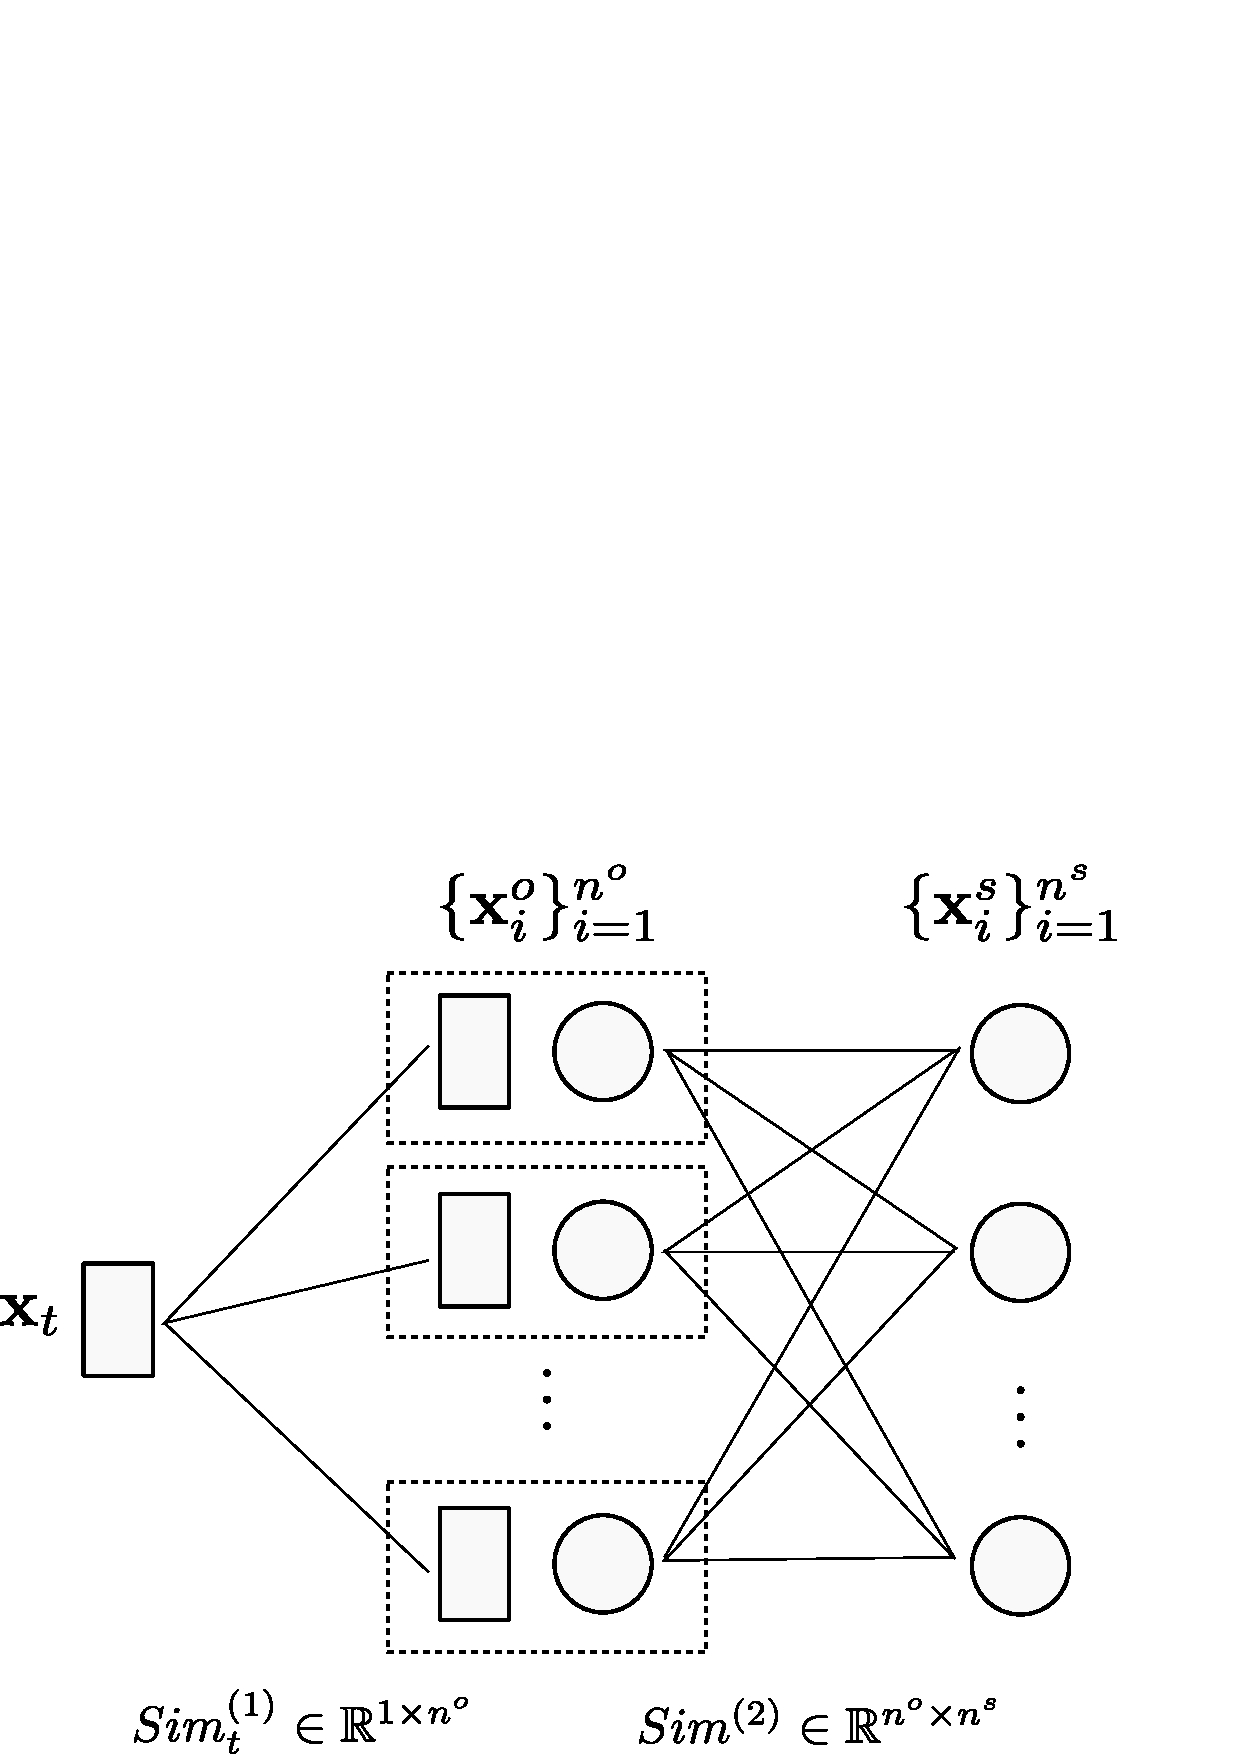
\includegraphics[height=0.15\textwidth]{knowledgetransfer.pdf}
\end{figure}
Similarity between $\mathbf{x}_t$ and each instance in the heterogeneous source domain
$$ Sim_t(j) = \sum\limits_i Sim_{t}^{(1)}(i) Sim^{(2)}(i,j) $$
Weighted $K$ nearest neighbor classifier
$$ h_{t}^{s}(\mathbf{x}_t) = \sum\limits_{i \in N} \frac{Sim_t(i)}{\sum\limits_{i \in N} Sim_t(i)} y_i $$
where $N$ is the set of identifiers of $K$ nearest neighbors in the heterogeneous source domain.
\end{frame}

\begin{frame}{Online Heterogeneous Transfer Algorithms}
\begin{columns}
\begin{column}{0.5\textwidth}
\begin{algorithm}[H]
\begin{algorithmic}[1]
\caption{Online Heterogeneous Transfer Algorithm 1 (OHT1)}
\algsetup{linenosize=\tiny}
\scriptsize
\REQUIRE ~~
aggressiveness parameter $C>0$\\ 
%~~~~~~~~~discount parameter $\beta \in (0,1)$\\ 
~~~~~~~~~$\eta = \frac{1}{2}$ \\
~~~~~~~~~heterogeneous source data
\ENSURE ~~
$\mathbf{v} = \mathbf{0}$, $w_{1}^{s} \in (0,1)$, $w_{1} \in (0,1)$, where $w_{1}^{s} + w_1 = 1$
\FOR{$t=1$ to $T$}
\STATE 
  receive instance: $\mathbf{x}_t \in \mathcal{X}$
\STATE
  normalize: $\theta_{t}^{s} = \frac{w_{t}^{s}}{w_{t}^{s}+w_t}, \theta_{t} = \frac{w_{t}}{w_{t}^{s}+w_t}$
\STATE
  predict: $\hat{y}_t = \sign \big( \theta_{t}^{s} \varOmega (h_{t}^{s}(\mathbf{x}_t)) + \theta_{t} \varOmega (\mathbf{v}_t \cdot \mathbf{x}_t) - \frac{1}{2} \big)$
\STATE
  receive correct label: $y_t \in \mathcal{Y}$
\STATE
  compute: 
    $$w_{t+1}^{s} = w_{t}^{s} \exp \big\{ -\eta \big(\varOmega(h_{t}^{s}(\mathbf{x}_t)) - \varOmega(y_t)\big)^2 \big\} $$
    $$w_{t+1} = w_{t} \exp \big\{ -\eta \big(\varOmega(\mathbf{v}_t \cdot \mathbf{x}_t) - \varOmega(y_t)\big)^2 \big\} $$
\STATE
  suffer loss: $\ell_{t}^{*} = \max \{0, 1-y_t(\mathbf{v}_t \cdot \mathbf{x}_t)\}$
\STATE
  set: $\tau_t = \frac{\ell_{t}^{*}}{{\|\mathbf{x}_t\|}^2}$
\STATE
  update: $ \mathbf{v}_{t+1} = \mathbf{v}_t + \tau_t y_t \mathbf{x}_t $
\ENDFOR
\end{algorithmic}
\end{algorithm}
where $\varOmega(z) = \max \{ 0, \min \{ 1, \frac{z+1}{2} \}\}$.
\end{column}
\begin{column}{0.5\textwidth}
\begin{algorithm}[H]
\begin{algorithmic}[1]
\caption{Online Heterogeneous Transfer Algorithm 2 (OHT2)}
\algsetup{linenosize=\tiny}
\scriptsize
\REQUIRE ~~
aggressiveness parameter $C>0$\\ 
~~~~~~~~~discount parameter $\alpha \in (0,1)$\\ 
~~~~~~~~~heterogeneous source data 
\ENSURE ~~
$\mathbf{v} = \mathbf{0}$, $w_{1}^{s} \in (0,1)$, $w_{1} \in (0,1)$, where $w_{1}^{s} + w_1 = 1$
\FOR{$t=1$ to $T$}
\STATE 
  receive instance: $\mathbf{x}_t \in \mathcal{X}$
\STATE
  normalize: $\theta_{t}^{s} = \frac{w_{t}^{s}}{w_{t}^{s}+w_t}, \theta_{t} = \frac{w_{t}}{w_{t}^{s}+w_t}$
\STATE
  predict: $\hat{y}_t = \sign \big( \theta_{t}^{s} \sign (h_{t}^{s}(\mathbf{x}_t)) + \theta_{t} \sign (\mathbf{v}_t \cdot \mathbf{x}_t) \big)$
\STATE
  receive correct label: $y_t \in \mathcal{Y}$
\STATE
  compute: 
    $$w_{t+1}^{s} = w_{t+1}^{s} \alpha ^ {I(y_t h_{t}^{s}(\mathbf{x}_t) \leq 0)}  $$
    $$w_{t+1} = w_{t+1} \alpha ^ {I(y_t (\mathbf{v}_t \cdot \mathbf{x}_t) \leq 0)}  $$
\STATE
  suffer loss: $\ell_{t}^{*} = \max \{0, 1-y_t(\mathbf{v}_t \cdot \mathbf{x}_t)\}$
\STATE
  set: $\tau_t = \frac{\ell_{t}^{*}}{{\|\mathbf{x}_t\|}^2}$
\STATE
  update: $ \mathbf{v}_{t+1} = \mathbf{v}_t + \tau_t y_t \mathbf{x}_t $
\ENDFOR
\end{algorithmic}
\end{algorithm}
Where indication function $I(\cdot)$ represents whether the hypothesis makes a wrong prediction or not.
\end{column}
\end{columns}
The equation of calculation of $\tau$ can be replaced by 
\begin{columns}
\begin{column}{0.5\textwidth}
$\tau_t = \min \{ C, \frac{\ell_{t}^{*}}{{\|\mathbf{x}_t\|}^2} \} $ 
\end{column}
\begin{column}{0.5\textwidth}
$ \tau_t = \frac{\ell_{t}^{*}}{{\|\mathbf{x}_t\|}^2 + \frac{1}{2C}} $ 
\end{column}
\end{columns}
\end{frame}

\section{Theoretical Analysis}
\begin{frame}{Theoretical Analysis}{$\mathbf{Hedge}(\beta)$ Algorithm}
At $t$-th trial, $\mathbf{Hedge}(\beta)$ algorithm synthesizes opinions from different experts based on a weight vector $\mathbf{weight}_t$, and updates the weight vector using rule
$$ weight_{t+1}^{i} = weight_{t}^{i} \cdot \beta^{loss_{t}^{i}} $$
where $\beta \in [0,1]$ and $loss_{t}^{i} \in [0,1]$.

\begin{tabular}{c|c|c}
\hline
\multicolumn{1}{c|}{$\mathbf{Hedge}(\beta)$} &
\multicolumn{1}{c|}{OHT1} &
\multicolumn{1}{c|}{OHT2} \\
\hline
$loss_{t}^{i}$ & $\ell_{t}^{s} = (\varOmega(h_{t}^{s}(\mathbf{x}_t)) - \varOmega(y_t)) ^ 2$ & $\ell_{t}^{s} = I(y_t h_{t}^{s}(\mathbf{x}_t) \leq 0)$ \\
               & $\ell_t = (\varOmega(\mathbf{v}_t \cdot \mathbf{x}_t) - \varOmega(y_t)) ^ 2$ & $\ell_{t} = I(y_t (\mathbf{v}_t \cdot \mathbf{x}_t) \leq 0)$ \\
\hline
$\beta$        & $\beta = \exp\{-\eta\}$ & $\beta = \alpha$ \\
\hline
\end{tabular}
OHT algorithms obey the rule of $\mathbf{Hedge}(\beta)$ algorithm.
\end{frame}

\begin{frame}{Theoretical Analysis}{Proposition}
\begin{prop}
%Let $\mathbf{L}_t = (\ell_{t}^{s}, \ell_{t})$ be the loss vector at $t$-th trial, and $\mathbf{W}_t = (\mathbf{w}_{t}^{s}, \mathbf{w}_{t})$ be the weight vector at $t$-th trial.
Given loss $\ell_{t}^{s} \in [0,1]$, $\ell_t \in [0,1]$ and decay factor $\beta \in (0,1)$, for any sequence of loss vectors $\{ (\ell_{t}^{s}, \ell_{t}) | t = 1, 2, \cdots T \} $, we have
$$ \sum\limits_{t=1}^{T} ( \theta_{t}^{s} \ell_{t}^{s} + \theta_t \ell_t ) \leq \frac{1}{1-\beta} \min \big( \varDelta^s, \varDelta \big) $$
where
$ \varDelta^s = \ln(\frac{1}{w_{1}^{s}}) + (\ln \frac{1}{\beta}) \sum\limits_{t=1}^{T} \ell_{t}^{s} $ and $ \varDelta = \ln(\frac{1}{w_{1}}) + (\ln \frac{1}{\beta}) \sum\limits_{t=1}^{T} \ell_{t} $
\end{prop}
\end{frame}

\begin{frame}{Theoretical Analysis}{Theorem}
\begin{thm}
Let $M$ be the number of mistakes made by OHT1 algorithm, then we have 
$$ M \leq \frac{4}{1-\beta} \min (\varDelta^s, \varDelta) $$
where
$ \varDelta^s = \ln(\frac{1}{w_{1}^{s}}) + (\ln \frac{1}{\beta}) \sum\limits_{t=1}^{T} \ell_{t}^{s} $ and $ \varDelta = \ln(\frac{1}{w_{1}}) + (\ln \frac{1}{\beta}) \sum\limits_{t=1}^{T} \ell_{t} $.
\end{thm}
\begin{thm}
Let $M$ be the number of mistakes made by OHT2 algorithm, then we have 
$$ M \leq \frac{2}{1-\beta} \min (\varDelta^s, \varDelta) $$
where
$ \varDelta^s = \ln(\frac{1}{w_{1}^{s}}) + (\ln \frac{1}{\beta}) \sum\limits_{t=1}^{T} \ell_{t}^{s} $ and $ \varDelta = \ln(\frac{1}{w_{1}}) + (\ln \frac{1}{\beta}) \sum\limits_{t=1}^{T} \ell_{t} $.
\end{thm}
\end{frame}

\section{Experiments}
\begin{frame}{Experiments}{Dataset}
NUS-WIDE dataset \\
\begin{itemize}
\item
~~Target domain: Image 
\item
~~Heterogeneous source: Text
\item
~~Co-occurrence data: co-occurred image-tag pairs
\end{itemize}
\end{frame}

\begin{frame}{Experiments}{Baseline Methods}
\begin{itemize}
\item
Passive-Aggressive algorithms \\
~~Do not exploit knowledge from the source domain
\item
Kernel function \\
~~Gaussian Kernel
\item
Number of nearest neighbors \\
~~$K$ = 100
\end{itemize}
\end{frame}

\begin{frame}{Experiments}{Results}
\begin{figure}
\centering
  \subfigure[PA-\uppercase\expandafter{\romannumeral2} vs. OHT1-\uppercase\expandafter{\romannumeral2}]
  {
    \label{11}
    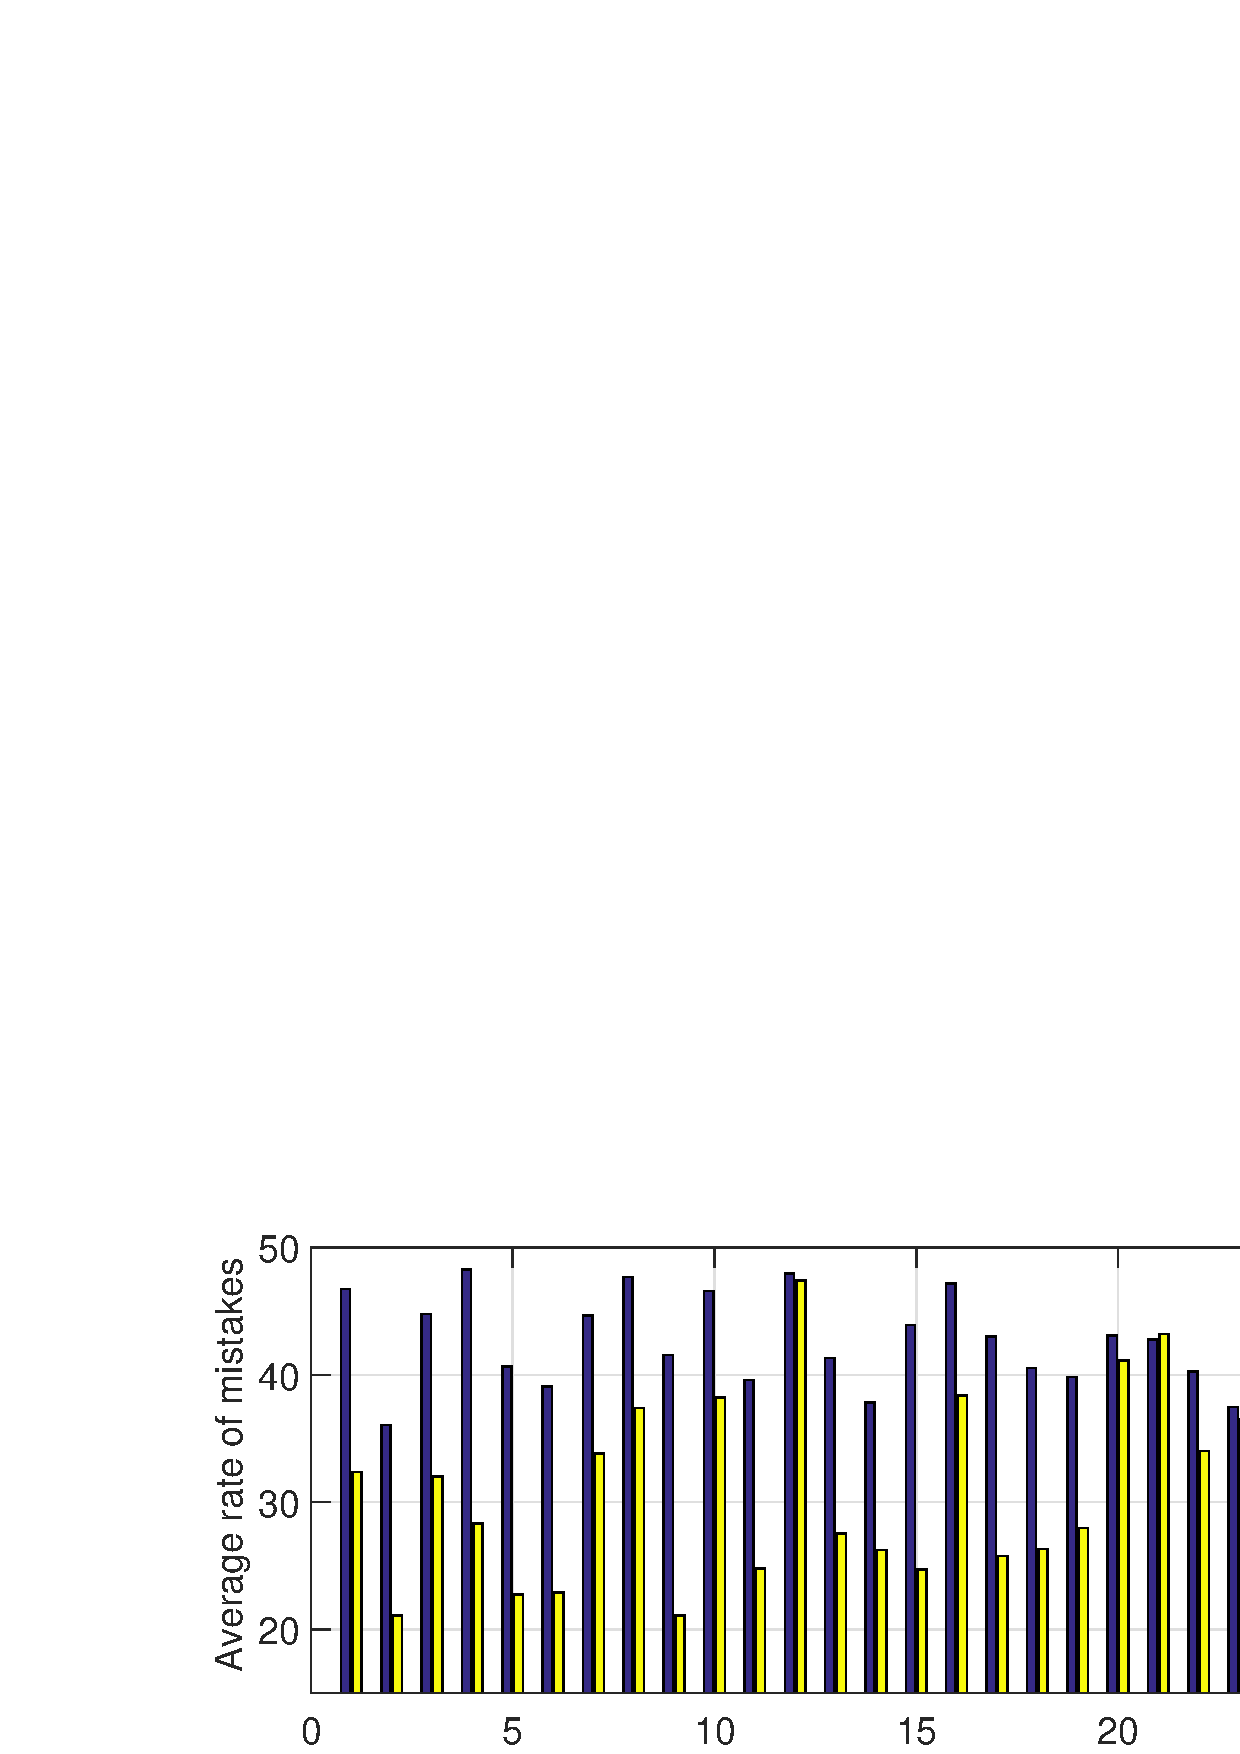
\includegraphics[width=18cm]{12_2.pdf}
  }
  \subfigure[PA-\uppercase\expandafter{\romannumeral2} vs. OHT2-\uppercase\expandafter{\romannumeral2}]
  {
    \label{12}
    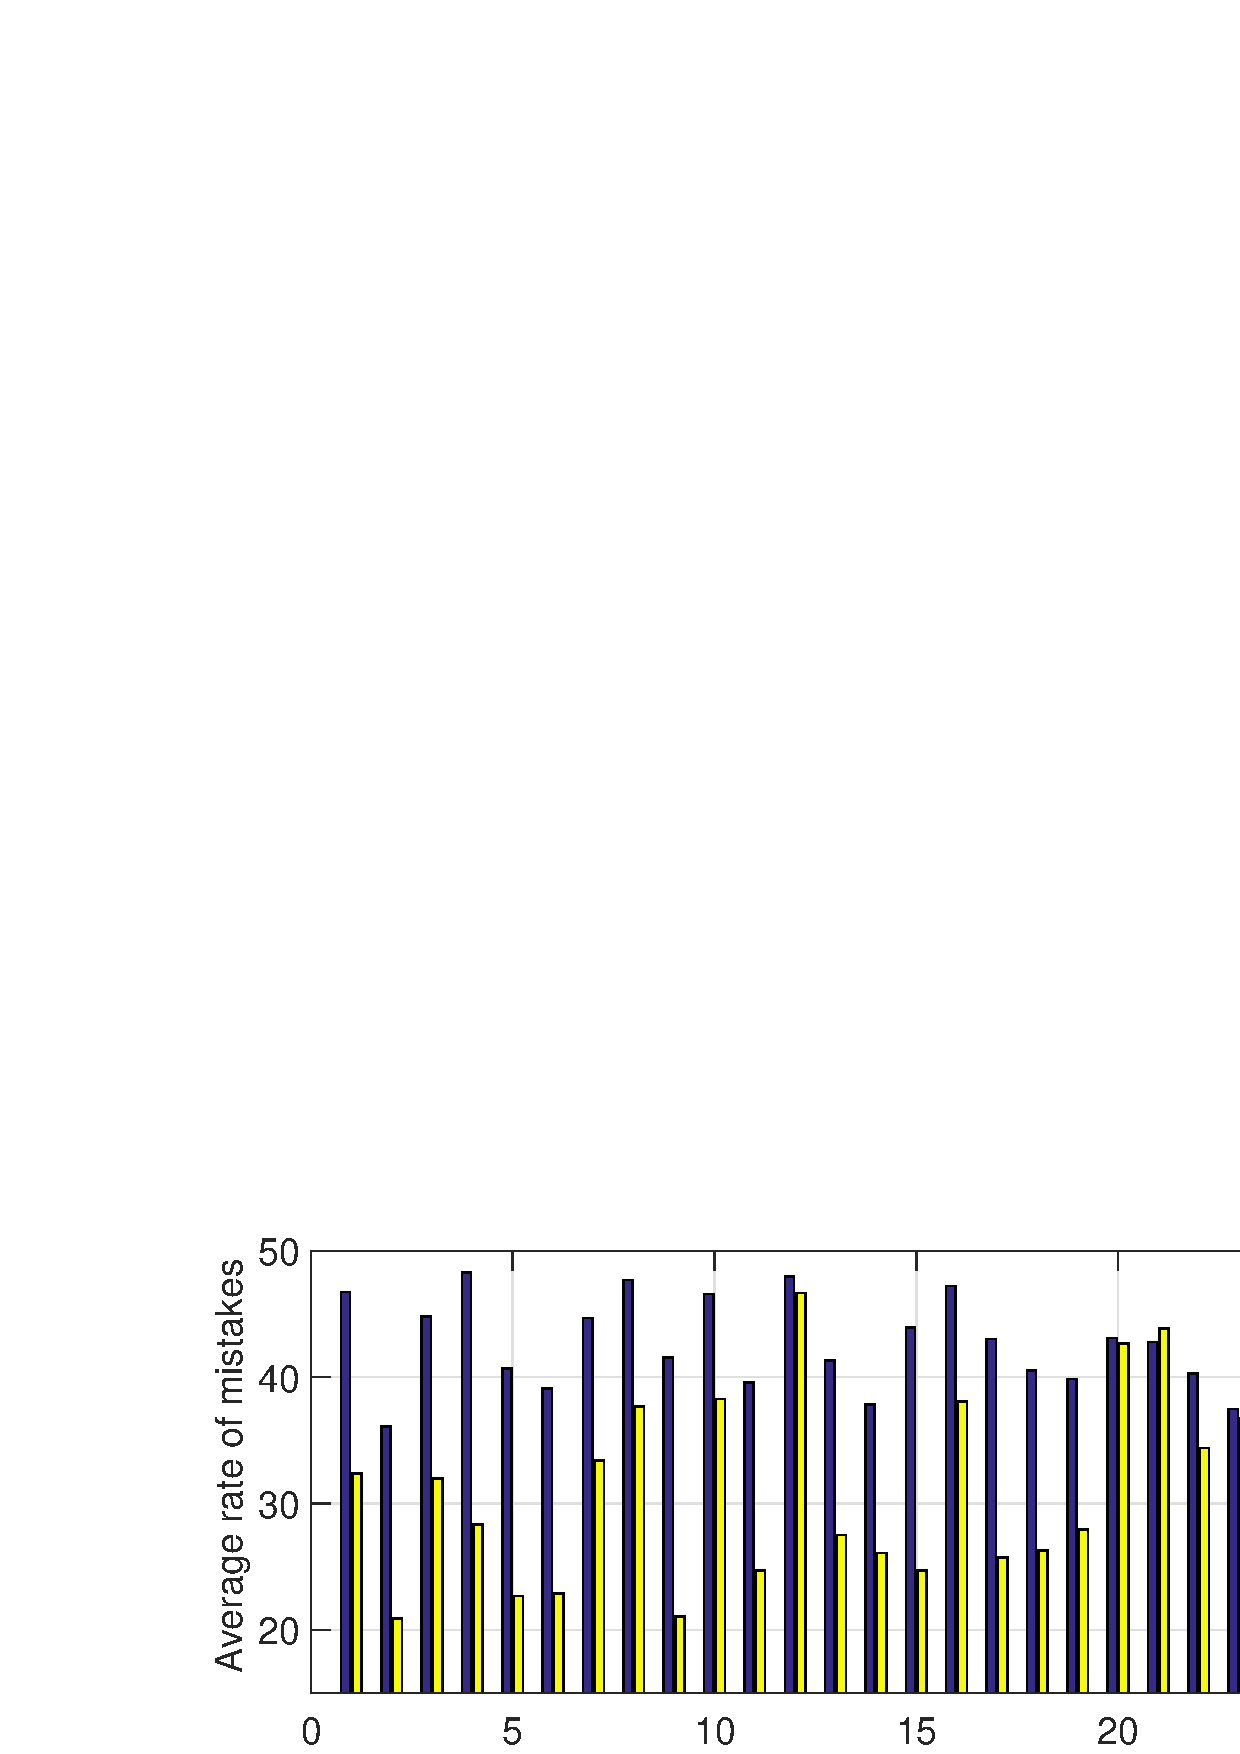
\includegraphics[width=18cm]{22_2.pdf}
  }
  \caption{Average rate of mistakes on all 45 tasks}
  \label{Average rate of mistakes on all 45 tasks}
\end{figure}
Observations:
\begin{itemize}
\item
The mistake rate of PA-\uppercase\expandafter{\romannumeral2} is very high.
\item
OHT methods generally outperform PA-\uppercase\expandafter{\romannumeral2}.
\end{itemize}
\end{frame}

\begin{frame}{Experiments}{Results}
\begin{figure}
\centering
  \subfigure[Task 2]
  {
    \label{task2}
    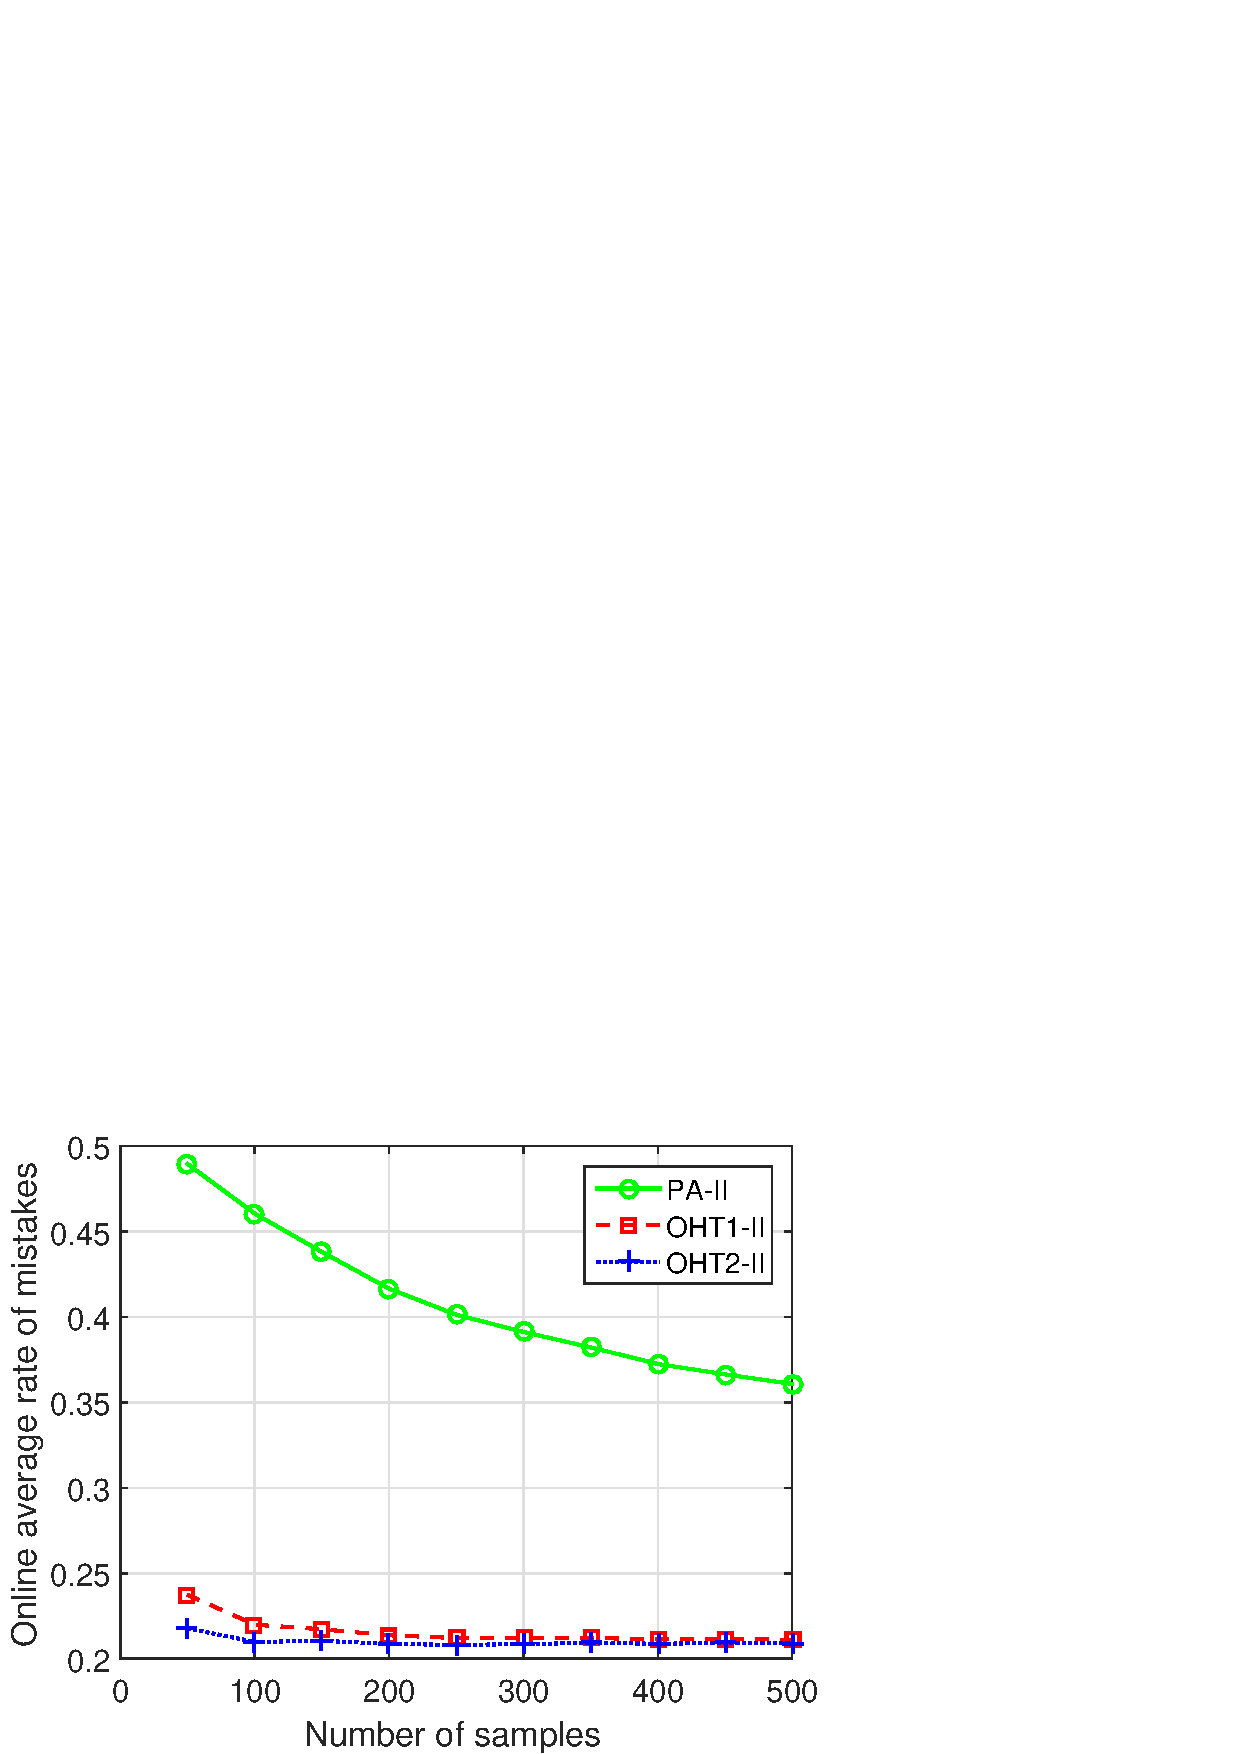
\includegraphics[width=5cm]{task2_2.pdf}
  }
  \subfigure[Task 14]
  {
    \label{task14}
    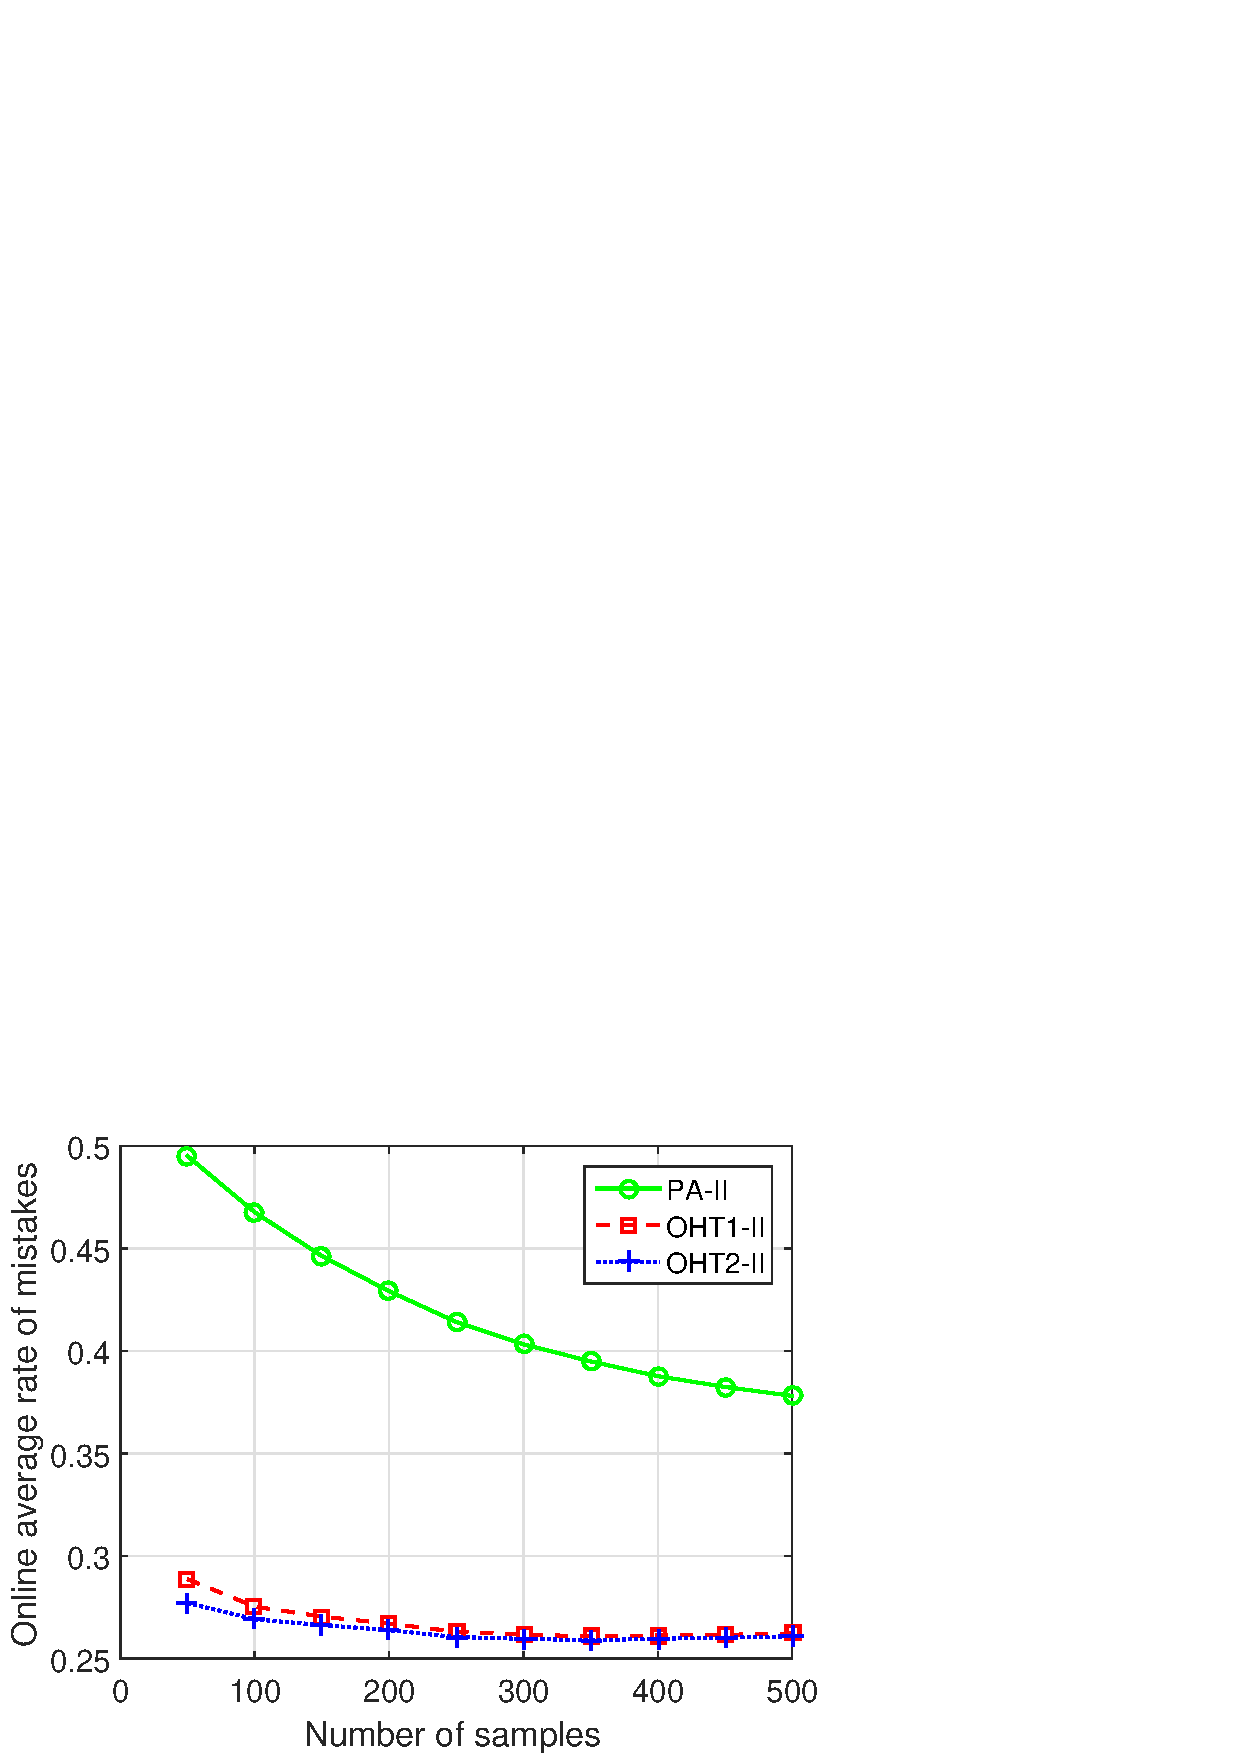
\includegraphics[width=5cm]{task14_2.pdf}
  }
  \subfigure[Task 36]
  {
    \label{task36}
    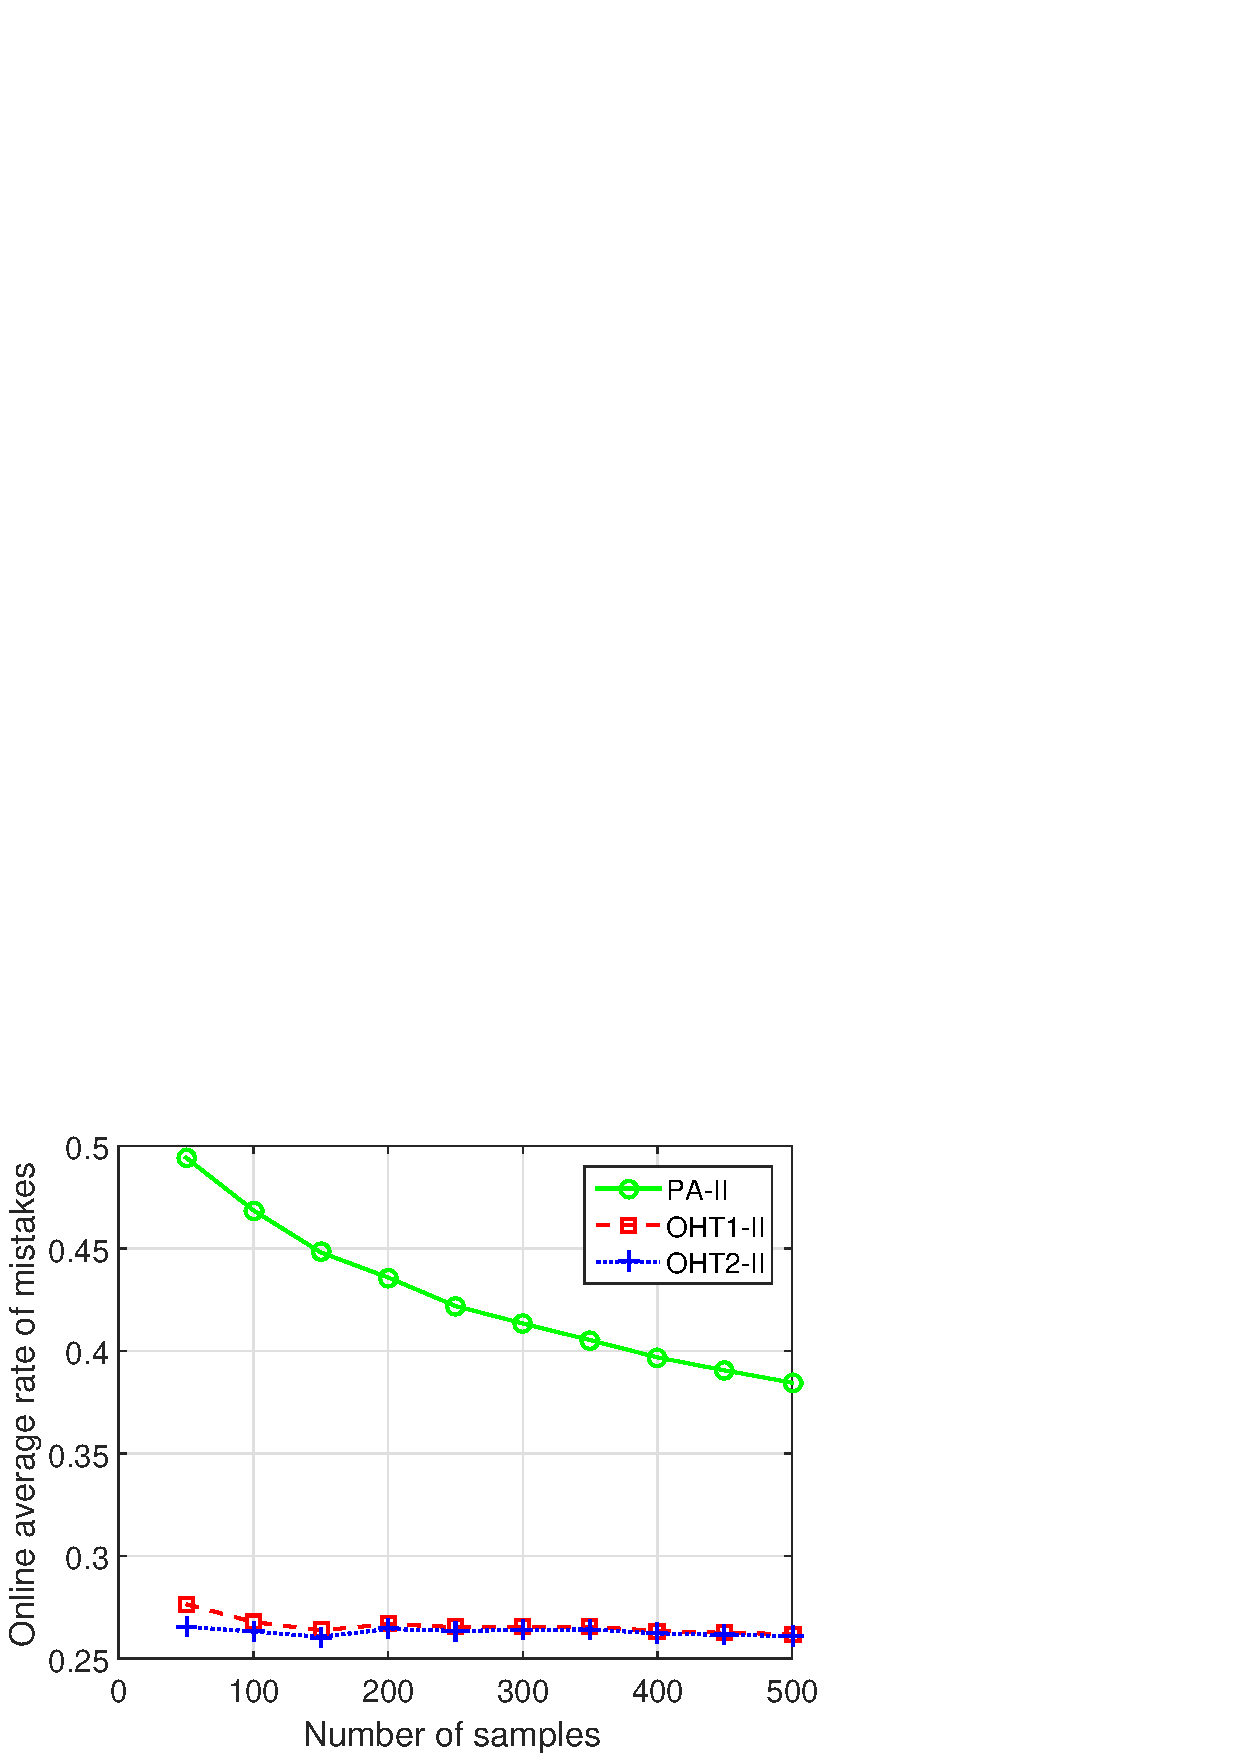
\includegraphics[width=5cm]{task36_2.pdf}
  }
  \\
  \subfigure[Task 7]
  {
    \label{task7}
    \includegraphics[width=5cm]{task7_2.pdf}
  }
  \subfigure[Task 16]
  {
    \label{task16}
    \includegraphics[width=5cm]{task16_2.pdf}
  }
  \subfigure[Task 33]
  {
    \label{task33}
    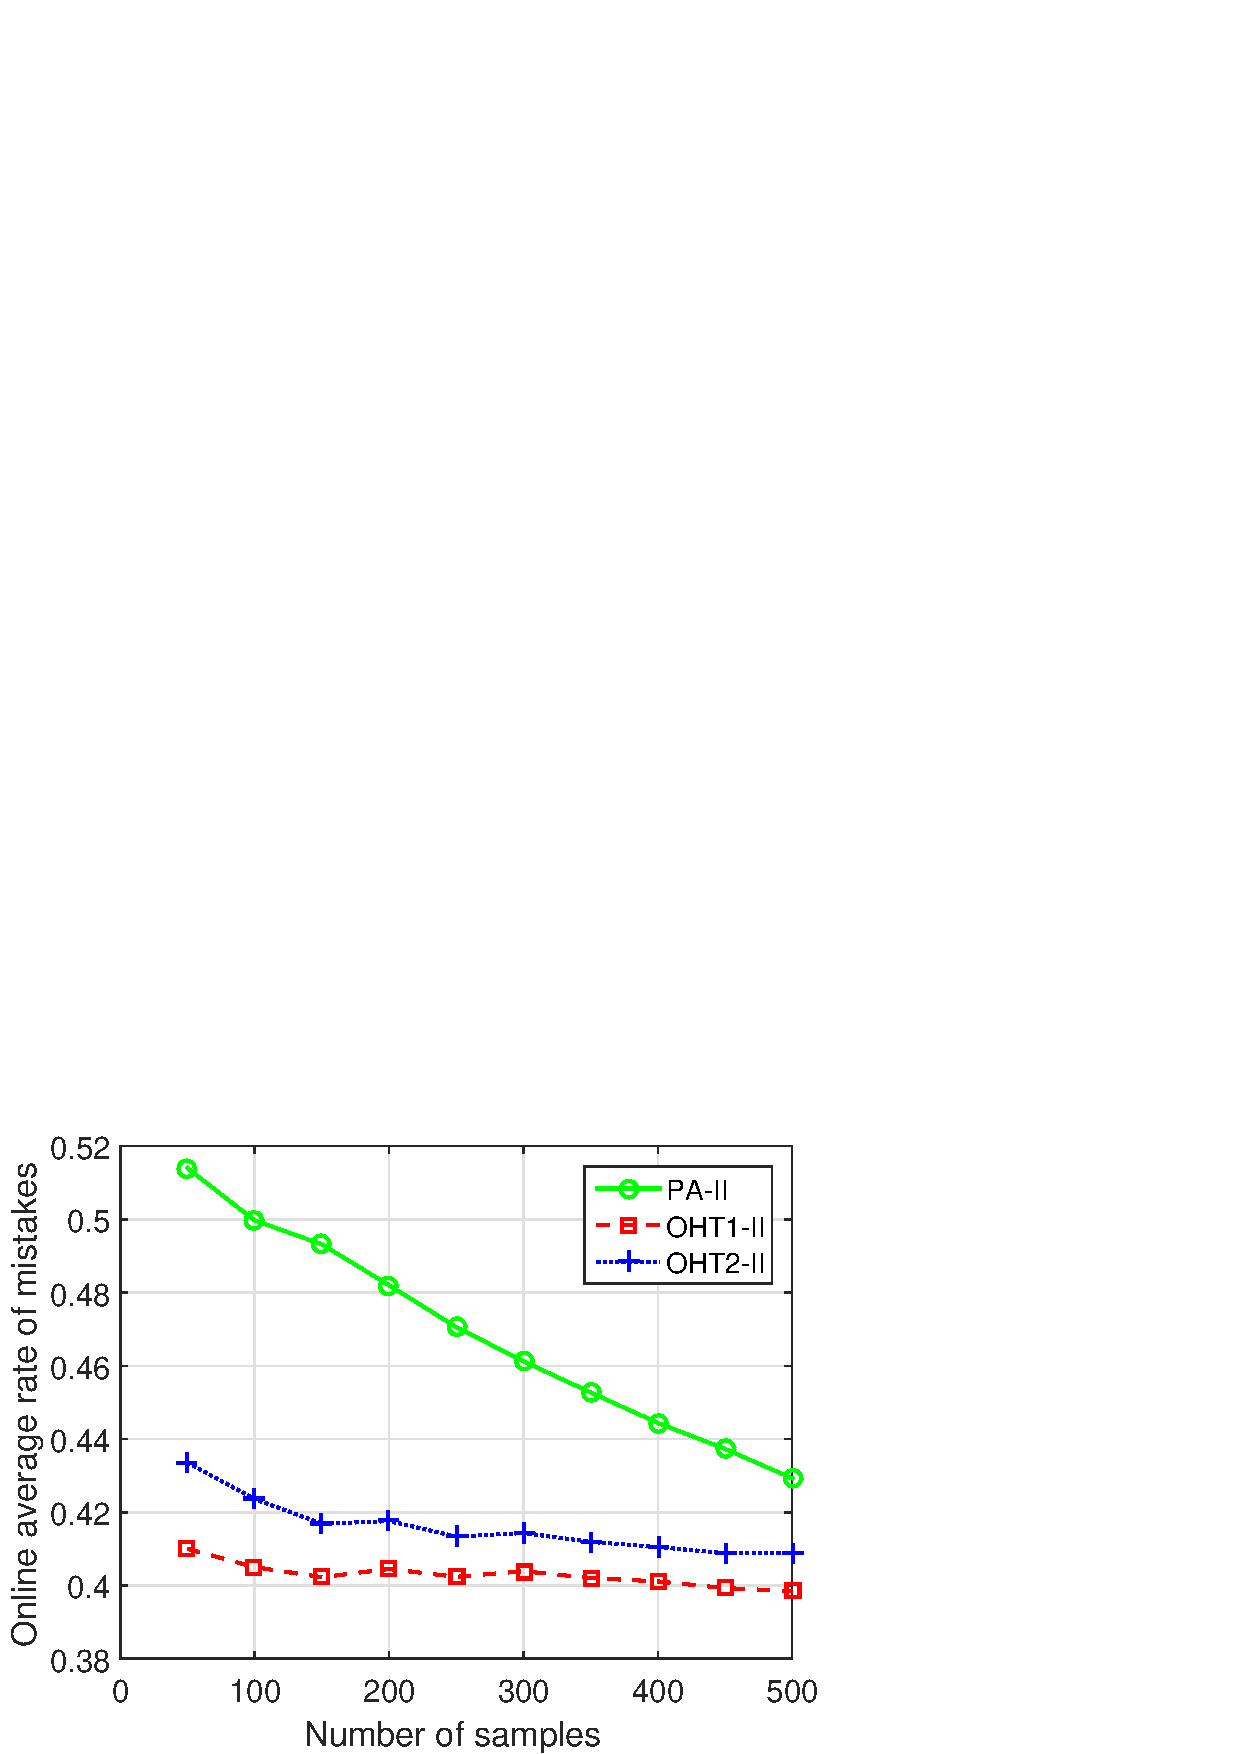
\includegraphics[width=5cm]{task33_2.pdf}
  }
  \caption{Online average rate of mistakes on example tasks}
  \label{Online average rate of mistakes on example tasks}
\end{figure}
Observations:
\begin{itemize}
\item
OHT algorithms usually achieve better performance at the beginning stage.
\item
On some tasks (e.g., 7, 16 and 33), the mistake rates of all algorithms decrease, but OHT methods always perform better.
\end{itemize}
\end{frame}

\begin{frame}{Experiments}{Significant Test}
Paired $t$-test ($\alpha = 0.01$)
\begin{itemize}
\item
OHT1 vs. PA: 44/0/1
\item
OHT2 vs. PA: 42/2/1
\end{itemize}
Cohen's $d$ value ( $d > 0.8$ : large promotion, $0.2 < d < 0.8$ : middle promotion)
\begin{itemize}
\item
OHT1: 41/3 
\item
OHT2: 40/3
\end{itemize}
\end{frame}

\begin{frame}{Experiments}{Parameters and Running Time}
\begin{figure}
\centering
  \subfigure[]
  {
    \label{average_error}
    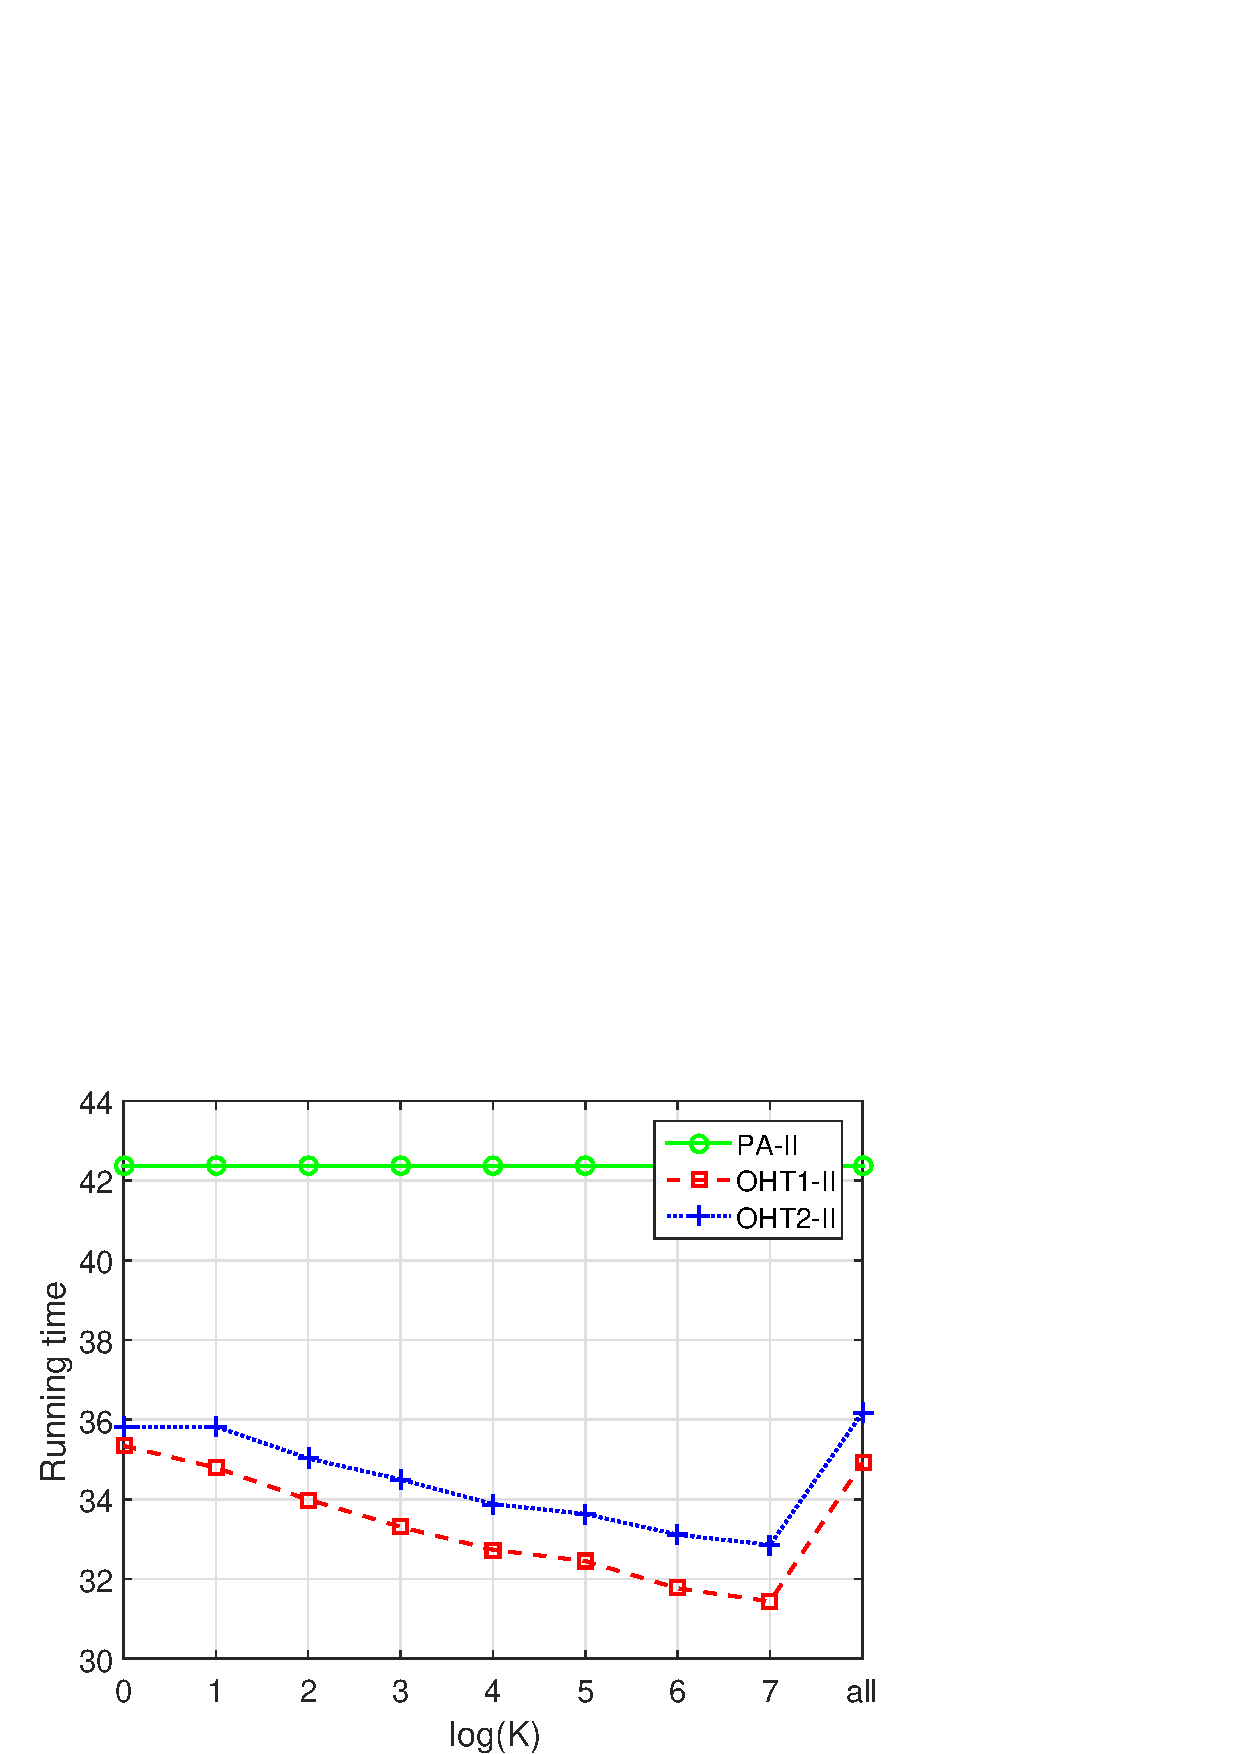
\includegraphics[width=3.5cm]{average_error.pdf}
  }
  \subfigure[]
  {
    \label{average_time}
    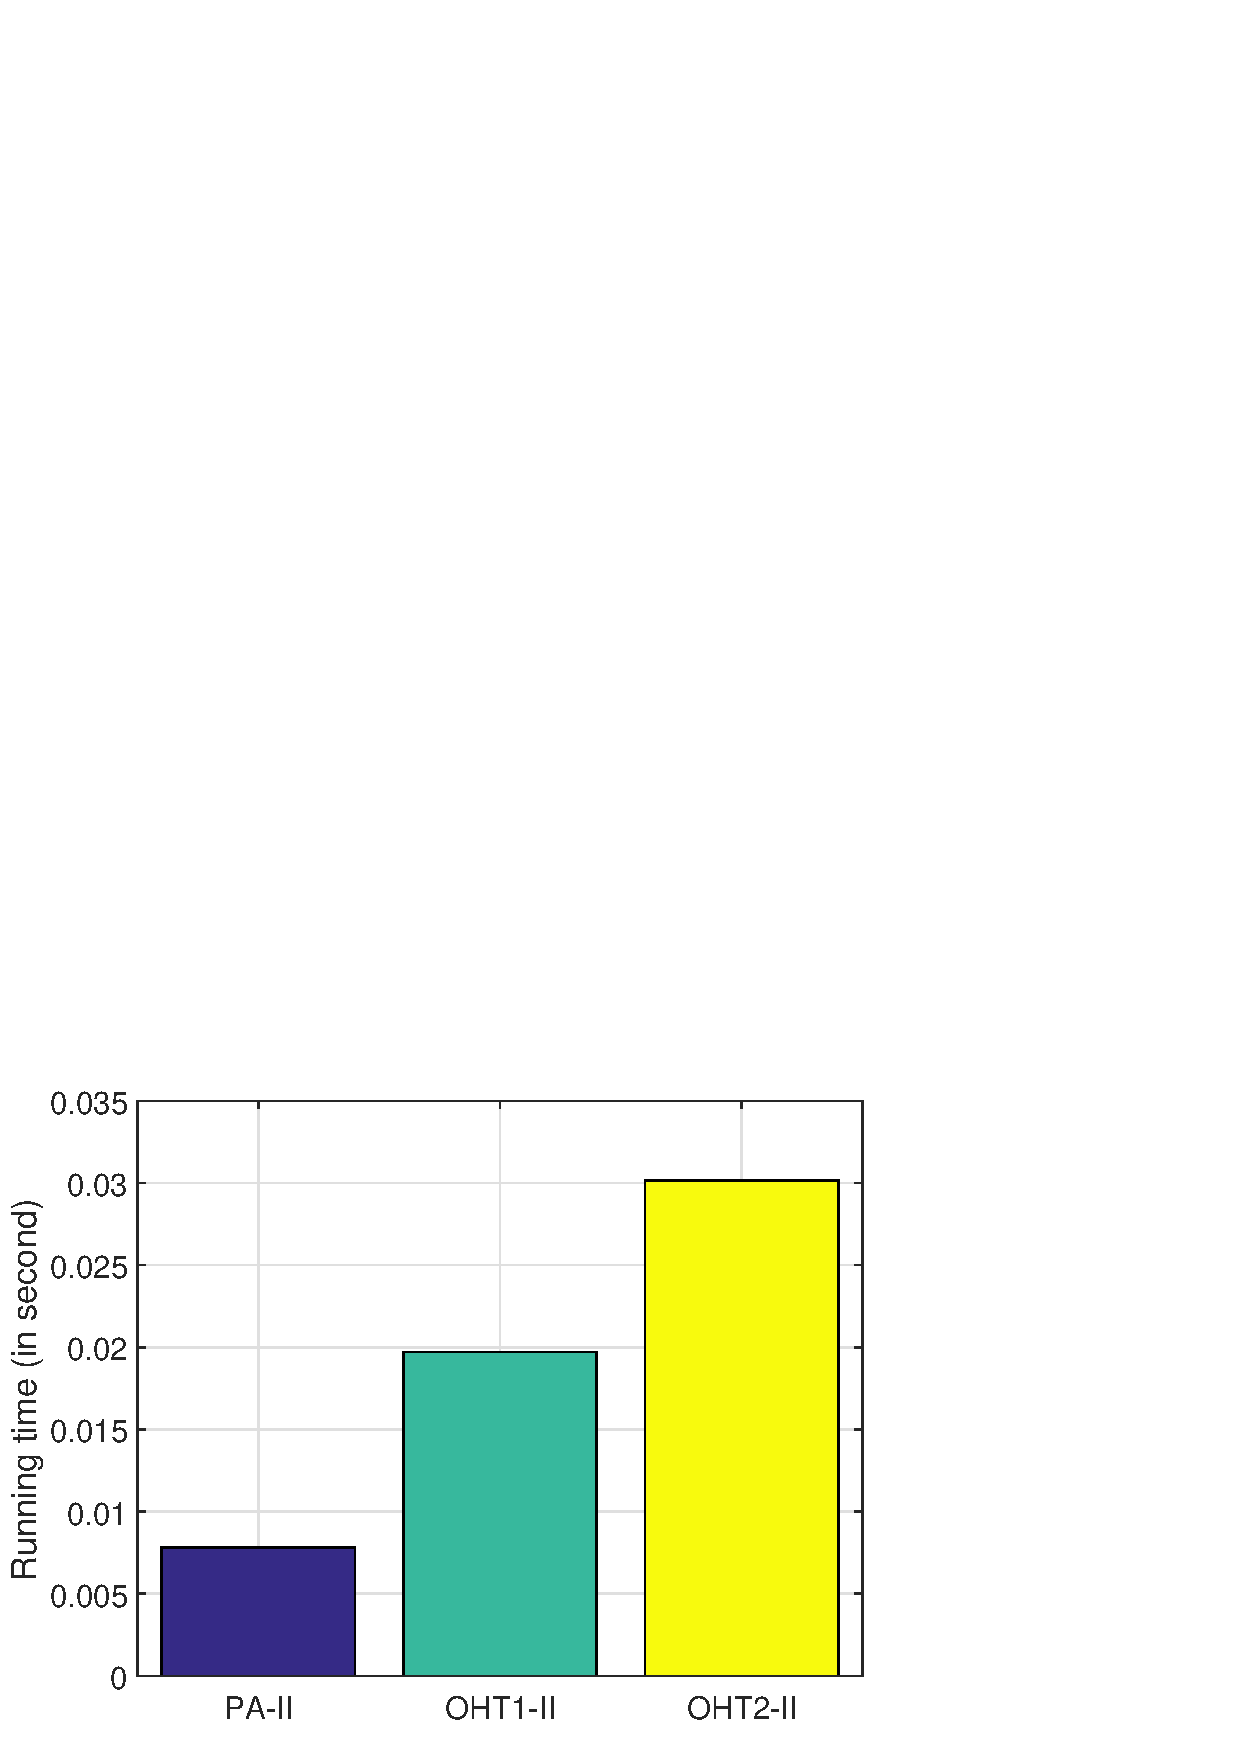
\includegraphics[width=3.9cm]{average_time.pdf}
  }
  \caption{(a) The average rate of mistakes under varying values of $K$. (b) The average running time of different algorithms when all instances in heterogeneous source are considered.}
  \label{average eok}
\end{figure}
\end{frame}

\section{Conclusion}
\begin{frame}{Conclusion}
\begin{itemize}
\item
We explore online heterogeneous transfer learning problem.
\item
We construct a connection across the domains using co-occurrence data, and apply the ensemble strategy to train a classifier.
\item
We offer the theoretical analysis of our algorithms.
\item
Experimental results show the effectiveness of our algorithms.
\end{itemize}
Future works:
\begin{itemize}
\item
applications with other types of data
\item
multiple source domains
\end{itemize}
\end{frame}

%\begin{frame}[allowframebreaks]{}
%\scriptsize
%\bibliographystyle{apacite}
%\bibliography{reference}
%\end{frame}

\section{}
\begin{frame}{}{}
\begin{center}
\begin{Huge}
$ \mathcal{THANK \ YOU}$ \\
$ \mathcal{FOR} $ \\
$ \mathcal{YOUR \ ATTENTION!}$ \\
\end{Huge}
\end{center}
\end{frame}

\end{document}


